\chapter{Preliminaries}

\section{Background on Dynamical Systems}

Throughout this thesis we study topological transformation groups, or in other words continuous group actions on topological spaces.
%
While these notions are rather standard, for the sake of completeness we provide all the required definitions here. We follow the treatment of \cite{deVries93} and \cite{GH55}. 
% 
From now on $G$ always denotes an infinite group and its identity element is denoted by $e$.

\begin{defn}[Topological transformation group]\label{def:dynamical_system}
A {\bf topological transformation group} is a triple $(X,G,\varphi)$, where $X$ is a compact metric space, $G$ is a countable discrete group and $\varphi$ is a continuous (left) group action of $G$ on $X$, that is,
\[
\varphi\colon G\times X \to X \quad 
\]
is a map satisfying the following conditions:
\begin{enumerate}
\item $\varphi(e,x)=x$ for all $x\in X$, 
\item $\varphi(g,\varphi(h,x))=\varphi(gh,x)$ for any $g,h\in G$ and $x\in X$,
\item $\varphi$ is continuous.
\end{enumerate}
If such a group action $\varphi$ of $G$ on $X$ is given, then we simply say that {\bf $\bm{G}$ acts on $\bm{X}$} or that $\varphi$ is a $\bm{G}${\bf-action} on $X$.
\end{defn}
\noindent

Note that since we restrict our attention to countable groups endowed with the discrete topology (countable discrete groups), the condition that $\varphi$ is continuous is equivalent to the fact that the map $g\mapsto \varphi(g,x)$ is continuous for every $g\in G$.



In the literature, there is a commonly agreed upon convention to denote a group action by $\cdot$ (dot) and use the infix notation, i.e., $\varphi(g,x) \equiv g\cdot x$.
%
Further, we often omit the dot, i.e., write $gx$ instead of $g\cdot x$ whenever this does not lead to confusion.
%
We also write $\bm{(X,G)}$ instead of $(X,G,\varphi)$.
%

Observe that a topological transformation group from Definition \ref{def:dynamical_system} naturally generalizes the standard notion of a discrete-time dynamical system $(X,T)$, where  $T:X\to X$ is a homeomorphism (see for instance \cite{HK95}). In this case the action $\cdot: \Z\times X \to X$ is defined as 
\[
 n\cdot x\defeq T^n(x)~~~~ \mbox{for $n\in\N$ and $x\in X$}.
\]
Notice that the above action $\cdot$ 
is an additive action of $\Z$ on $X$, which allows us to treat $(X,T)$ as a dynamical system $(X,\Z)$, i.e., a dynamical system generated by $\Z$.

In this thesis we use the name ``dynamical system'' as a synonym for ``topological transformation group''.

Let $(X,G)$ be a dynamical system.
%
For two subsets $S,T \subseteq G$ we often write $ST$ to denote the set $\{st: s\in S, t\in T\} \subseteq G$ of pairwise products, similarly we define $SA:=\{sx:s\in S,\,x\in A\}$ for $A\subseteq X$.
%
We denote the {\bf orbit} of an element ${x}\in X$ (with respect to a $G$-action) by
\[
Gx\defeq \{gx:g\in G\}
\]
and by $\und{x}_G\in X^G$, the {\bf trajectory} of ${x}$, i.e., $\und{x}_G(g)\defeq gx$ for all $g\in G$. 
%
Note that trajectory is a function $G\to X$, while the orbit is the set of the values attained by the trajectory.
%
We say that $x\in X$ is a {\bf fixed point} if $Gx=\{x\}$.
%
A subset $A\subseteq X$ is $\bm{G}${\bf-invariant} if $GA\subseteq A$. 
%
If $Y\subseteq X$ is a non-empty closed $G$-ivariant set, we say that $Y$ is a {\bf subsystem} of $X$.  
%
What follows is a quite simple, yet useful property of invariant sets:

\begin{lem}\label{lem:closed-inv}
Let $(X,G)$ be a dynamical system. If $A\subseteq X$ is invariant, then $\closure{A}$ (the closure of $A$) is invariant.
\end{lem}

\begin{proof}
Let $x\in\closure{A}$ and $g\in G$. There exist a sequence $\{x_n\}_{n\in\N}\subseteq A$ such that $x_n\to x$ ($n\to\infty$). Since $A$ is invariant, $gx_n\in A$ for every $n\in\N$. We also have $gx_n\to gx$ since $G$ acts on $X$ continuously. Therefore $gx\in\closure{A}$.
\end{proof}

\noindent
Observe that Lemma \ref{lem:closed-inv} implies that $\closure{Gx}$ is a subsystem of $X$ for every $x\in X$.

When $G$ acts on $X$ then this automatically gives rise to $G$-actions (i.e. actions of  $G$) on the space of functions $Y^X$ (for any set $Y$) and on the space of Borel probability measures $\M(X)$ on $X$ endowed with the weak-$\star$ topology. Formal definition of these actions follow
\begin{defn}[Induced Group Actions]\label{def:induced_group_action}
Suppose that $(X,G)$ is a dynamical system, then:
\begin{enumerate}
\item For an arbitrary set $Y$, the $G$-action induced on $Y^X$ is defined as follows: for any $\tau: X\to Y$ and $g\in G$ the function $(g\cdot \tau):X\to Y$  satisfies
\[
(g\cdot\tau)(x) \defeq \tau(g x) \quad\text{ for } x\in X.
\]
\item If $\mu \in \M(X)$ is any Borel probability measure on $X$ then the result of the action of an element $g\in G$ on $\mu$ is denoted by $g_{*}(\mu)$ and is given by
\[
g_*(\mu)(A)\defeq\mu(g^{-1} A)~~~~~~~~~\mbox{for any $A\in \mB(X)$,}
\]
where $\mB(X)$ denotes the collection of all Borel sets on $X$. This defines a dynamical system $(\M(X),G)$ on the compact space $\M(X)$.
\end{enumerate}
\end{defn}

\noindent
In this thesis the following classes of dynamical systems often show up and play an important role
\begin{defn}[Classes of dynamical stystems]
We say that a dynamical system $(X,G)$ is
\begin{enumerate}
\item {\bf transitive} if there exists an $x\in X$ such that $X=\closure{Gx}$;
\item {\bf minimal} if $X$ does not contain any non-empty, proper, closed $G$-invariant subset;
\item {\bf proximal} if $\displaystyle \inf_{g\in G}\rho(gx,gz)=0$ for every $x,z\in X$.
\end{enumerate}
\end{defn}

\noindent
As already mentioned, when it comes to $X$, we are mainly interested in compact metric spaces.
%
The only assumption on $G$ that we have made so far is that it is countable, now comes the second crucial assumption that allows us to study entropy and other familiar notions developed for dynamical systems generated by $\Z$, i.e., that $G$ is an amenable group.

\begin{defn}[Amenability]
We say that a countable group $G$ is {\bf amenable} if it admits  a {\bf \Folner sequence} $\{F_n\}_{n\in\N}$ in $G$ (where $\N=\{0,1,2,\ldots\}$), that is a sequence of non-empty finite subsets of $G$ satisfying 
\[
\lim_{n\to\infty}\frac{|gF_n\Delta F_n|}{|F_n|}= 0~~~~~~\mbox{for every $g\in G$,}
\]
where $\Delta$ denotes a symmetric difference.
\end{defn}

\noindent
For a thorough discussion on amenable groups, including a historical perspective, basic properties and examples, we refer to \cite{CC10}. 

From now on, without mentioning explicitly, we always assume that $\bm{X}$ {\bf is a compact metric space equipped with a metric $\bm{\rho}$} satifying\footnote{This is without loss of generality as a metric $\rho$ can be always replaced by the equivalent metric $\mathrm{min}(\rho,1)$.} $\bm{\rho(x,z)\leq 1}$ for $x,z\in X$ and $\bm{G}$ {\bf is a discrete countable amenable group}.
%
Amenable groups are especially important in the context of dynamical systems since they allow to naturally generalise the notion of topological entropy from classical dynamical systems (i.e., $(X,T)$ where  $T\colon X\to X$ is a continuous map) to dynamical systems generated by arbitrary (amenable) group actions. Entropy is the central invariant in the study of these actions and can be defined for an action of an amenable group $G$ (with a \Folner sequence $\{F_n\}_{n\in \N}$) on a space $X$ as follows:
%
\begin{defn}[Topological entropy]\label{def:entropy}
For a finite open cover $\mathcal U$ of the space $X$ let $\mathcal N(\mathcal U)$ be the minimum cardinality of a subcover of $\mathcal U$. Define the join of two finite open covers $\mathcal U$ and $\mathcal V$ as
\[
\mathcal U\vee\mathcal V\defeq\{U\cap V\colon U\in\mathcal U, V \in\mathcal V\}.
\]
Given $F=\{f_1,\ldots,f_s\}\subseteq G$ and $f\in F$ we write 
\[ f^{-1}\mathcal U\defeq \{f^{-1}U\colon U\in \mathcal U\} \quad\text{and} \quad\mathcal U^F \defeq (f_1^{-1}\mathcal{U})\vee\ldots\vee (f_s^{-1}\mathcal{U}).\] By $h(X, \mathcal U)$ we denote the limit of the sequence 
$\displaystyle
\inbrace{\frac{\log\mathcal N\inparen{\mathcal U^{F_n}}}{|F_n|}}_{n\in\N}.
$
\\
The {\bf topological entropy} of $(X,G)$ is defined as 
\[
\htop(X)\defeq\sup\{h(X,\mathcal U)\,:\,\mathcal U\text{ is an open cover of }X\}.
\]
Further, for any element $x\in X$ its entropy is defined as  $h(x)\defeq\htop(\closure{Gx})$.
\end{defn}

\noindent
Observe that $\vee$ is an associative operation on open covers thus $\cU^F$ is well-defined.
%
Moreover, note that for the above definition to make sense, one must show existence of $h(X, \cU)$. It is also not at all clear that $h(X,\cU)$ does not depend on the choice of a \Folner sequence $\{F_n\}_{n\in\N}$. Indeed, the existence of $h(X,\cU)$ as well as its independence of the choice of the \Folner sequence follows from \cite[Theorem 6.1]{LW00} (see Lemma~\ref{lem:LW}).





%-------------------------------------------------

\section{Shift Spaces}
Even though many of our results apply to the general case, when $X$ is a compact, metric space, an important case that is of special focus is the Cantor space, i.e., when $X=\alf^G$ (the space of all functions $G\to \alf$), where $\alf$ is a finite discrete metric space, called an {\bf alphabet}. A standard way to define a metric $\rho$ on $\alf^G$ that induces the Tychonoff product topology on $\alf^G$ is
\begin{equation}\label{eq:cantorMetric}
\rho(z,y)\defeq |\alf|^{-k}\quad\text{ with } \quad k\defeq  \min\inbrace{i\in\N: z(g_i)\neq y(g_i)},
\end{equation}
where $(g_1,g_2,\ldots)$ is any bijective enumeration of elements of $G$. An especially important family of subsets of $\alf^G$ are cylinders:

\begin{defn}[Cylinder]\label{def:cylinder}
For a finite set $F\subseteq G$ and $w\in\alf^F$, we define a {\bf cylinder} in $\alf^G$ by
\[
[w]_F = \{x\in\alf^G: x_F = w\},
\]
where $x_F = x\restrict{F}$. If $a\in\alf$ and $F=\{g\}$ for some $g\in G$, we denote for simplicity
\[
[a]_g = \{x\in\alf^G: x(g) = a\}.
\]
\end{defn}
\noindent
We recall also that the cylinders are both open and closed in the topology induced by $\rho$ and thus $\alf^G$ endowed with $\rho$ has a base consisting of clopen sets.
%
A group action that is perhaps the most natural to consider in such symbolic spaces is \emph{the shift}

\begin{defn}[Shift action]
Given $\alf$, we define the {\bf shift action} $(\alf^G,G)$ as the following action of $G$ on $\alf^G$:
\[
\varphi\colon G\times \alf^G \to \alf^G \quad \text{ (with the standard notation } \varphi(g,x)=g\cdot x),
\]
where
\[
(g\cdot x)(h) = x(hg) \quad \mbox{ for $h\in G$ and $x\in\alf^G$}.
\]
\end{defn}

\noindent
Notice that such defined shift action is compatible with what one would think a shift is supposed to be in the case of $G=\Z$, i.e., it moves a sequence $x\in\alf^{\Z}$ one place to the left, formally
\[
\sigma\colon \alf^{\Z}\to\alf^{\Z} ~~~~~~\text{ satisfying }~~~~~~ \sigma(x)(n) = x(n+1).
\] 
Closed, non-empty, invariant subspaces of a shift space are called {\bf subshifts}.





\section{Groups}\label{section:groups}
We review a few notions related to groups as well as define certain classes of groups that are of particular interest in this thesis.
% 
We start by a definition of a \emph{monotile} that allows us to study ``periodic'' sets that appear in connection with minimal and proximal dynamical systems. It was widely studied in \cite{Weiss01}.

\begin{defn}[Monotile]\label{def:tile}
A (right) {\bf monotile}  of $G$ is a finite set $F\subseteq G$ such that $e\in F$ and $\{Fc: c\in C\}$ is a partition of $G$ for some $C\subseteq G$, i.e., the following two conditions are satisfied:
\begin{enumerate}
\item $\displaystyle \bigcup_{c\in C} Fc = G;$
\item $Fc_1\cap Fc_2=\emptyset$ for $c_1,c_2\in C$ with $c_1\neq c_2$.
\end{enumerate}
We also say that $C$ is  a {\bf set of centers} associated with $F$.
\end{defn}

\noindent
Note that the set $\{e\}$ is a monotile in every group. Moreover, it is important to realize, that a set of centers associated with a given monotile $F$ does not need to be unique.
\begin{example}[A monotile with uncountably many sets of centers]
Let $G=\Z\times\Z_2$. Then the set $F=\inbrace{(0,0),(0,1)}$ is a monotile and for every $\{i_n\}_{n\in\Z}\in\{0,1\}^{\Z}$, the set $\{(n,i_n):n\in\Z\}$ is a set of centers associated with $F$.
\end{example}

\noindent
It is not known whether every amenable group admits a \Folner sequence whose elements are monotiles, but it is clearly the case for $G=\Z$ or more generally $G=\Z^n$. This motivates the following definition, which was first introduced in \cite{CC19} and generalizes the concept of amenable residually finite groups.

\begin{defn}[Congruent monotileable group]\label{def:congruent_monotilable}
A countable amenable group $G$ is  {\bf congruent monotileable} if it admits a \Folner sequence $\F=\{F_n\}_{n\in\N}$ satisfying:
\begin{enumerate}
\item $F_0=\{e\}$,
\item $\displaystyle\bigsqcup_{h\in J_n}F_nh=F_{n+1}$ for some  $J_n\subseteq G$ with $e\in J_n$ for every $n\in\N$ ,
\item $\bigcup\F=G.$
\end{enumerate}
If the above conditions hold, then we also say that $\F$ is a {\bf congruent \Folner sequence}.
\end{defn}
\noindent
We show that every congruent monotileable group $G$ has an \emph{elegant structure} (see Figure \ref{fig:tree} and Lemma \ref{lem:elegant_C_n}) that allows to define a periodic configuration over $G$.

\begin{lem}[Unique factorization]\label{lem:factorization}
Let $G$ be a congruent monotileable group and let  $\F=\{F_n\}_{n\in\N}$ be a congruent \Folner sequence in $G$. If sets $\{J_n\}_{n\in\N}$ in $G$ are such that for every $n\in\N$ it holds 
\[
 e\in J_n~~~~~~\text{ and }~~~~~~\bigsqcup_{h\in J_n}F_nh=F_{n+1},
\]   
then for every $g\in G$, there exists a unique element
$
(h_0,h_1,h_2,\ldots)\in J_0\times J_1\times J_2\times\ldots
$
such that $h_i=e$ for all but finitely many $i\in\N$ and 
$
g=h_0h_1h_2\ldots.
$
\end{lem}

\begin{proof}
Fix $g\in G$. First we justify the existence of a factorization of $g$. 
Since $\bigcup\F=G$, there exists $N\in\N$ such that $g\in F_N$. 
%
We set $h_n=e$ for $n\geq N$.
%
We can also find $f_{N-1}\in F_{N-1}$ and $h_{N-1}\in J_{N-1}$ such that 
\[
g=f_{N-1}h_{N-1}.
\]
Again, there are $f_{N-2}\in F_{N-2}$ and $h_{N-2}\in J_{N-2}$ such that 
\[
g=f_{N-2}h_{N-2}h_{N-1}.
\]
Proceeding inductively, we obtain elements $h_i\in J_i$ for $i=0,1,\ldots,N-1$ such that (since $F_0=\{e\}$)
\[
g=h_0h_1\ldots h_{N-1}.
\]
To see that this representation is unique, observe that the condition 
\[
\bigsqcup_{h\in J_n}F_nh=F_{n+1} ~~~~~~\text{ for every } n\in\N
\]
implies that for every $n\in\N$  and for every $f_1,f_2\in F_n$ and $h_1,h_2\in J_n$ it holds 
\[
f_1h_1 = f_2h_2~~~~\implies ~~~~ f_1=f_2 \mbox{ and } h_1=h_2,
\]
thus the sequence $(h_0, h_1,h_2,\ldots)$ is unique.
\end{proof}


\begin{figure}
\centering
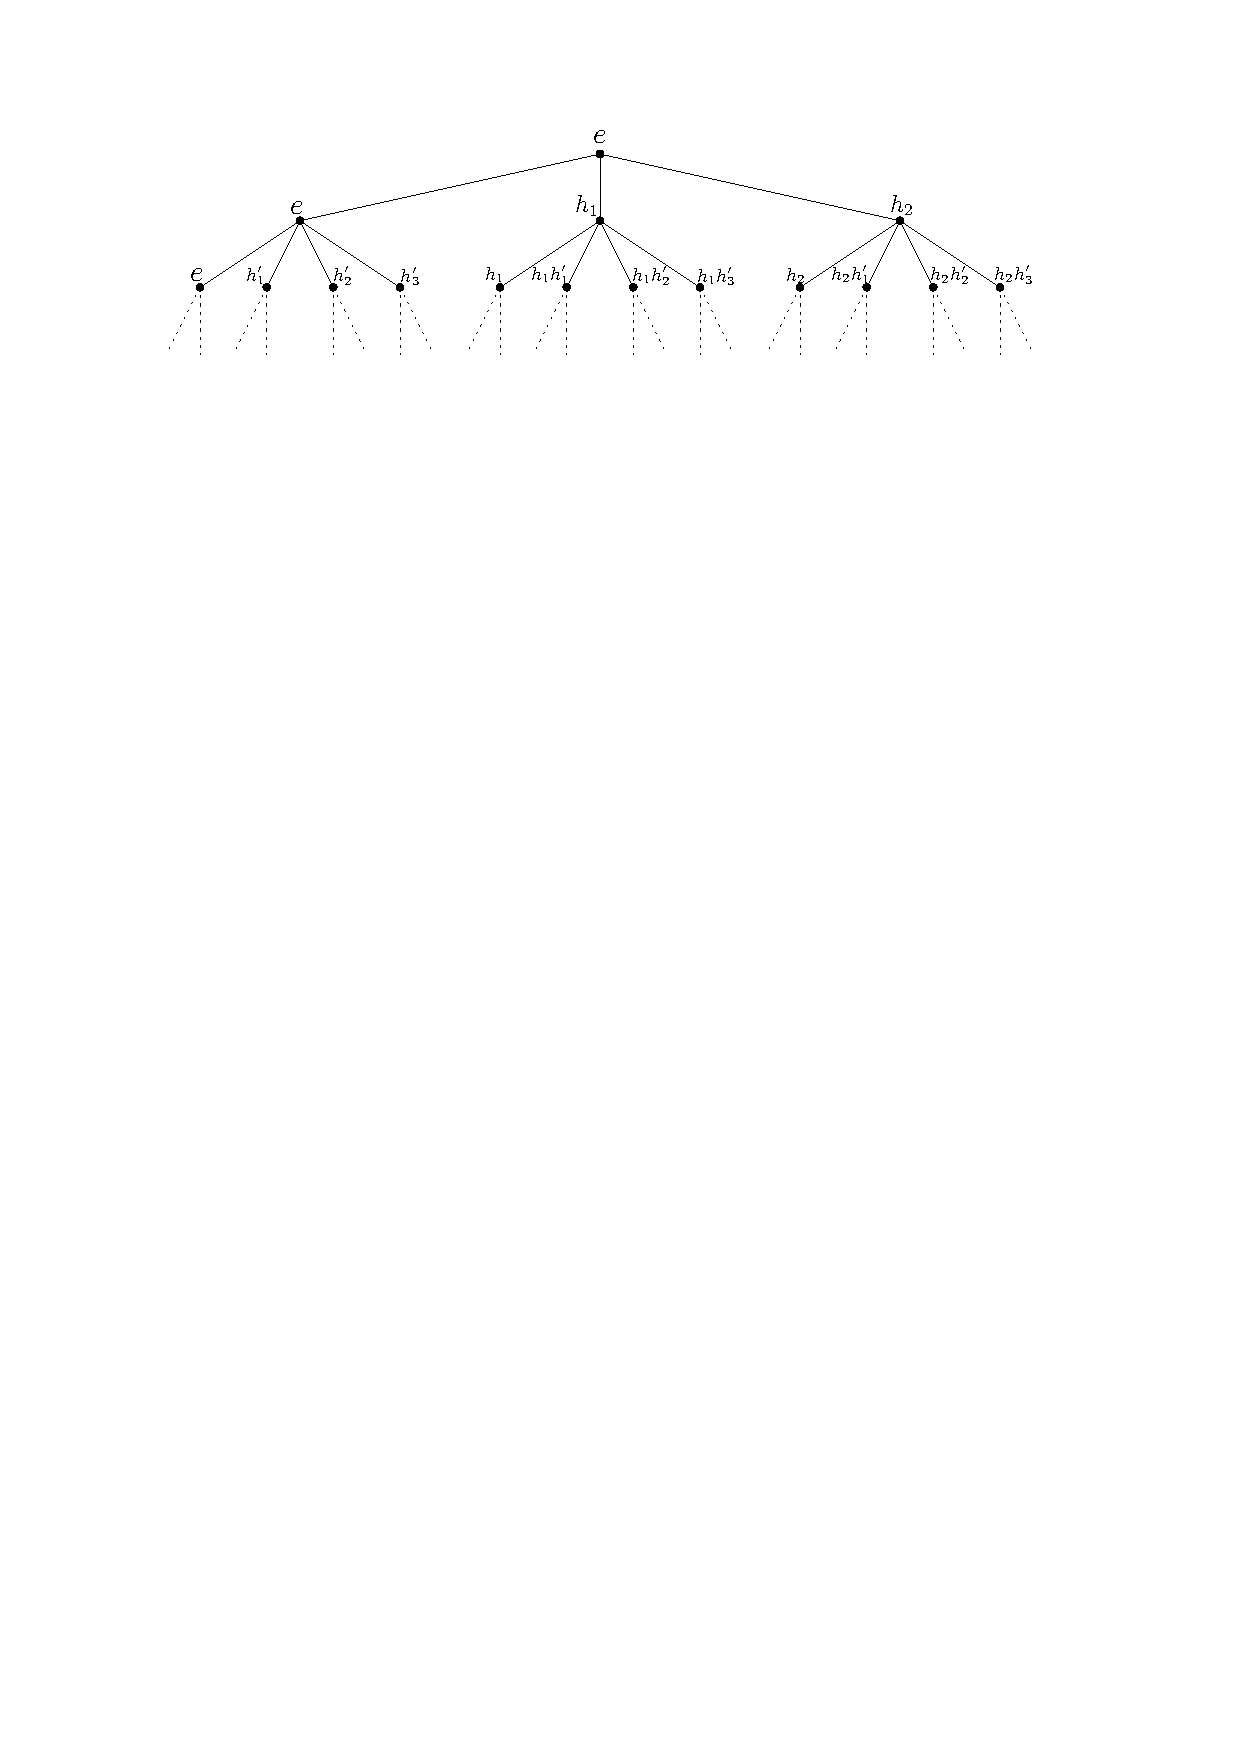
\includegraphics[scale=1]{Graphics/tree_representation2}
\caption{The proof of Lemma \ref{lem:elegant_C_n} shows us the structure of a congruent monotileable group $G$ from a new perspective. We can think of $G$ as a tree $T$ such that every vertex is identified with some element of $G$ according to the congruent \Folner sequence $\{F_n\}_{n\in\N}$ and  sets $\{J_n\}_{n\in\N}$ from Definition \ref{def:congruent_monotilable}. The figure depicts a sample tree $T$ for $J_0=\{e,h_1,h_2\}$ and  $J_1=\{e,h'_1,h'_2,h'_3\}$. We construct $T$ as follows: 
we set $e$ to be the root of $T$. If $g\in G$ is a vertex of depth $n\in\N$, then we define its children as elements $gh$ for $h\in J_n$. Then observe that $F_n$ corresponds to the set of all vertices at depth $n$. For example $F_1 = \{e,h_1,h_2\}$. Moreover if $f\in F_n$, then $fC_n$ is the set of all vertices of the full subtree of $T$ rooted in $f$. For example $h_1C_1$ is the set $\{h_1,h_1,h_1h'_1,h_1h'_2,h_1h'_3,\ldots \}$.}\label{fig:tree}
\end{figure}

\noindent
As a consequence of a unique factorization of elements of $G$ given by sets $J_n$ (for $n\in\N$), we obtain sets of centers associated with $\F$ that has all nice properties required for the construction of a quasi-Toeplitz configuration (see Lemma \ref{lem:connected1}).

\begin{lem}\label{lem:elegant_C_n}
Let $G$ be a congruent monotileable group. Fix  $\F=\{F_n\}_{n\in\N}$ a congruent \Folner sequence in $G$ with sets $\{J_n\}_{n\in\N}$ as in Definition \ref{def:congruent_monotilable}. Then there exist a sequence $\mC=\{C_n\}_{n\in\N}$ in $G$ such that for every $n\in\N$ the following conditions hold
\begin{enumerate}
\item $C_n$ is an associated with $F_n$ set of centers,
\item $J_n\subseteq C_n$,
\item $\displaystyle C_n=\bigsqcup_{h\in J_n}hC_{n+1}$.
\end{enumerate}
We say that $\mC$ is the {\bf \elegant sequence of centers} associated with $\F$.
\end{lem}

\begin{proof}
Fix $n\in\N$. Observe that if $n\geq 1$, then
\[
F_n = \inbrace{h_0h_1\ldots h_{n-1}: h_i\in J_i \text{ for every } i=0,1,\ldots,n-1 }.
\]
For $n\geq 1$ we define
\[
C_n\defeq\inbrace{h_nh_{n+1}h_{n+2}\ldots: h_i\in J_i \text{ for every } i\in\N_{\geq n} \text{ and } h_i=e \text{ for almost all } i\in\N_{\geq n} }.
\]
Notice that the condition $3$ follows directly from the definition of $C_n$. It is also clear that $J_n\subseteq C_n$ since $e\in J_i$ for every $i\in\N$. Moreover, by Lemma \ref{lem:factorization} we have guaranteed that $F_nC_n=G$ and $F_nc\cap F_n \tilde{c}=\emptyset$ for every $c,\tilde{c}\in C_n$ such that $c\neq\tilde{c}$.
\end{proof}

\noindent
It is worth emphasizing that from Lemma \ref{lem:elegant_C_n} we obtain that if $\{F_n\}_{n\in\N}$ is a congruent \Folner sequence, then $F_n$ is a monotile for every $n\in\N$.

As we have already mentioned, the notion of congruent monotileable group generalizes the concept of amenable residually finite group.

\begin{defn}[Residually finite group]\label{def:res_fin}
A countable group $G$ is \emph{residually finite} if there exists a sequence $\{H_n\}_{n\in \N}$ of finite index normal subgroups satisfying:
\begin{enumerate}
\item $H_n\supseteq H_{n+1}$ for every $n\in\N$,
\item $\displaystyle \bigcap_{n\in\N} H_n = \{e\}.$
\end{enumerate}  
\end{defn}
\noindent
Recall that the index of a subgroup $H$ in $G$ is defined as the number of cosets of $H$ in $G$, that is, the number $|\{gH:g\in G\}|$. We write $H\triangleleft_f G$ if $H$ is a finite index normal subgroup of $G$.

It was proved in \cite{CP14} that if a group is amenable and residually finite, then there exists a special \Folner sequence associated to a sequence of finite index normal subgroups $\{H_n\}_{n\in\N}$.

\begin{lem}\label{Cortez}\cite[Lemma 4]{CP14}
If $G$ is an amenable residually finite group then there exist
a sequence $\{H_n\}_{n\in \N}$ with $H_n\lhd_f G$ and  a F{\o}lner sequence $\{F_n\}_{n\in\N}$ satisfying:
\begin{enumerate}
\item $\displaystyle G=H_0\supseteq H_1\supseteq H_2\supseteq\ldots\text{ and }\bigcap_{n=0}^{\infty}H_n=\{e\},$
\item $\displaystyle\{e\}=F_0\subseteq F_1\subseteq F_2\subseteq\ldots\text{ and }\bigcup_{n=0}^{\infty}F_n=G,$
\item\label{problem} $\displaystyle F_{i+1}=\bigsqcup_{h\in F_{i+1}\cap H_{i}}F_ih\text{ for every }i\in\N$,
\item for every $n\in\N$ the set $F_n$ is a fundamental domain for $G/H_{n}$, that is, $|F_n|=\inmodul{G/H_n}$ and $\{fH_n:f\in F_n\}=\{gH_n:g\in G\}$.
\end{enumerate}
\end{lem}

\begin{figure}
\centering
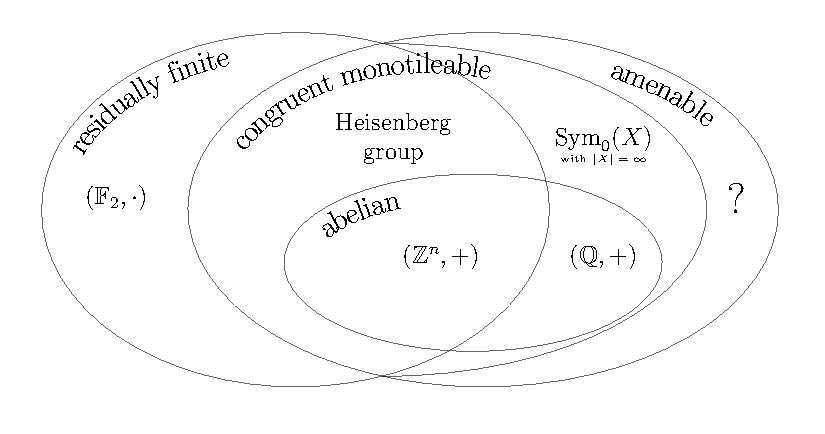
\includegraphics[scale=1]{Graphics/grupy}
\caption{A diagram depicting inclusions between different classes of countable groups considered in this thesis. Congruent monotileable groups are a generalisation of residually finite amenable groups. It is not known whether every amenable group is congruent monotileable (this is denoted by a question mark in the diagram). The free group generated by two elements is denoted by $\mathbb{F}_2$. The group $\text{Sym}_0(X)$ is the group of all permutations of $X$ with finite support, where the support of permutation $\pi$ of $X$ is the set $\{x\in X : \pi(x)\neq x \}$. For the proof that every abelian group is coungruent monotileable see \cite{CC19}.}\label{fig:groups}
\end{figure}

\noindent
Therefore if $G$ is amenable and residually finite and $\F=\{F_n\}_{n\in \N}$ is given by Lemma \ref{Cortez}, then $\F$ satisfies the conditions from Definition \ref{def:congruent_monotilable} hence $G$ is a congruent monotileable group.
%
Now, the relation between amenable residually finite groups and congruent monotileable groups is clear: a set of centers associated with a given element of a \Folner sequence plays the role of a finite index normal subgroup in a group that is not necessarily residually finite. 
%
They give us some form of regularity in a group, but such a structure is not as nice as the one induced by a subgroup of finite index.


In Figure~\ref{fig:groups} we show how the classes of groups defined in this section relate to each other with respect to the inclusion.
%-----------------------------------------------------------------------------



